%%%%%%%%%%%%%%%%%%%%%%%%%%%%%%%%%%%%%%%%%%%%%%%%%
% IIIT Lucknow M.Tech Thesis — Progress Report
% Title: AI Voice Sales Agent + CRM Automation
% Author: Jatin Saini (MSA24023)
%%%%%%%%%%%%%%%%%%%%%%%%%%%%%%%%%%%%%%%%%%%%%%%%%

\documentclass[12pt,a4paper,oneside]{book}

% ===== Packages =====
\usepackage[utf8]{inputenc}
\usepackage[T1]{fontenc}
\usepackage{times}
\usepackage[top=1in, bottom=1in, left=1.5in, right=1in]{geometry}
\usepackage{graphicx}
\usepackage{amsmath,amssymb,amsfonts}
\usepackage{setspace}
\usepackage{titlesec}
\usepackage{fancyhdr}
\usepackage{hyperref}
\usepackage{url}
\usepackage{booktabs}
\usepackage{longtable}
\usepackage{tabularx}
\usepackage{multirow}
\usepackage{enumitem}
\usepackage{listings}
\usepackage{xcolor}
\usepackage{caption}
\usepackage{subcaption}
\usepackage{algorithm}
\usepackage{algpseudocode}
\usepackage{tikz}
\usepackage{float}
\usepackage{natbib}
\usepackage[acronym,toc]{glossaries}

% ===== Line spacing =====
\onehalfspacing

% ===== Hyperref setup =====
\hypersetup{
    colorlinks=true,
    linkcolor=black,
    citecolor=blue,
    urlcolor=blue,
}

% ===== Code listing style =====
\lstdefinestyle{codestyle}{
    backgroundcolor=\color{gray!10},
    commentstyle=\color{green!60!black},
    keywordstyle=\color{blue!80!black}\bfseries,
    stringstyle=\color{red!70!black},
    basicstyle=\ttfamily\footnotesize,
    breakatwhitespace=false,
    breaklines=true,
    captionpos=b,
    keepspaces=true,
    numbers=left,
    numbersep=5pt,
    numberstyle=\tiny\color{gray},
    showspaces=false,
    showstringspaces=false,
    showtabs=false,
    tabsize=2,
    frame=single,
    rulecolor=\color{gray!50},
}
\lstset{style=codestyle}

% ===== Header/Footer =====
\pagestyle{fancy}
\fancyhf{}
\fancyhead[L]{\leftmark}
\fancyfoot[C]{\thepage}
\renewcommand{\headrulewidth}{0.4pt}

% ===== Abbreviations =====
\newacronym{ai}{AI}{Artificial Intelligence}
\newacronym{ml}{ML}{Machine Learning}
\newacronym{crm}{CRM}{Customer Relationship Management}
\newacronym{api}{API}{Application Programming Interface}
\newacronym{tts}{TTS}{Text-to-Speech}
\newacronym{asr}{ASR}{Automatic Speech Recognition}
\newacronym{sdk}{SDK}{Software Development Kit}
\newacronym{sip}{SIP}{Session Initiation Protocol}
\newacronym{voip}{VoIP}{Voice over Internet Protocol}
\newacronym{nlp}{NLP}{Natural Language Processing}
\newacronym{rest}{REST}{Representational State Transfer}
\newacronym{ui}{UI}{User Interface}
\newacronym{csv}{CSV}{Comma-Separated Values}

\makeglossaries

\begin{document}

%%%%%%%%%%%%%%%%%%%%%%%%%%%%%%%%%%%%%%%%%%%%%%%%%
% COVER PAGE
%%%%%%%%%%%%%%%%%%%%%%%%%%%%%%%%%%%%%%%%%%%%%%%%%
\begin{titlepage}
\centering
\vspace*{1cm}

{\LARGE\bfseries AI Voice Sales Agent with CRM Automation:\\A Cloud-Based Automated Outbound Calling System}

\vspace{2cm}

{\Large\bfseries M.Tech}

\vspace{2cm}

{\Large\bfseries Jatin Saini\\(MSA24023)}

\vspace{2.5cm}

\includegraphics[width=0.3\textwidth]{iiitl_logo}

\vspace{0.5cm}

{\large\bfseries DEPARTMENT OF COMPUTER SCIENCE\\
INDIAN INSTITUTE OF INFORMATION TECHNOLOGY,\\
LUCKNOW\\
2023 -- 2025}

\end{titlepage}

% Blank page after cover
\newpage\thispagestyle{empty}\mbox{}\newpage

%%%%%%%%%%%%%%%%%%%%%%%%%%%%%%%%%%%%%%%%%%%%%%%%%
% INNER TITLE PAGE
%%%%%%%%%%%%%%%%%%%%%%%%%%%%%%%%%%%%%%%%%%%%%%%%%
\begin{titlepage}
\centering
\vspace*{0.5cm}

\rule{\textwidth}{1pt}
\vspace{0.3cm}

{\LARGE\bfseries AI Voice Sales Agent with CRM Automation:\\A Cloud-Based Automated Outbound Calling System}

\vspace{0.3cm}
\rule{\textwidth}{1pt}

\vspace{1cm}

\textit{A thesis submitted in partial fulfillment of the requirements for the award of the degree of}

\vspace{0.5cm}

{\large\bfseries M.Tech.}\\
in\\
{\large\bfseries Computer Science (AI \& ML)}

\vspace{1cm}

by

\vspace{0.5cm}

{\large\bfseries Jatin Saini\\(MSA24023)}

\vspace{1cm}

under the guidance of

\vspace{0.5cm}

{\large\bfseries Dr. Sersindu Barman}

\vspace{1.5cm}

\includegraphics[width=0.25\textwidth]{iiitl_logo}

\vspace{0.3cm}

{\large\bfseries Indian Institute of Information Technology, Lucknow\\
2023--25}

\vspace{0.3cm}

{\small \copyright\ Indian Institute of Information Technology, Lucknow 2025.}

\end{titlepage}

\newpage\thispagestyle{empty}\mbox{}\newpage

%%%%%%%%%%%%%%%%%%%%%%%%%%%%%%%%%%%%%%%%%%%%%%%%%
% DEDICATION
%%%%%%%%%%%%%%%%%%%%%%%%%%%%%%%%%%%%%%%%%%%%%%%%%
\thispagestyle{empty}
\vspace*{5cm}
\begin{center}
\textit{To}\\
\textit{My family and mentors, whose unwavering support\\
and encouragement made this work possible}
\end{center}
\newpage\thispagestyle{empty}\mbox{}\newpage

%%%%%%%%%%%%%%%%%%%%%%%%%%%%%%%%%%%%%%%%%%%%%%%%%
% AUTHORSHIP
%%%%%%%%%%%%%%%%%%%%%%%%%%%%%%%%%%%%%%%%%%%%%%%%%
\chapter*{AUTHORSHIP}
\addcontentsline{toc}{chapter}{Authorship}

I, \textbf{Jatin Saini}, declare that this thesis titled, ``\textbf{AI Voice Sales Agent with CRM Automation: A Cloud-Based Automated Outbound Calling System}'' and the work presented in it are my own. I confirm that:

\begin{itemize}
    \item This work was completed entirely while in candidature for Master of Technology degree at Indian Institute of Information Technology, Lucknow.
    \item Where I have consulted the published work of others, it is always cited.
    \item Wherever I have cited the work of others, the source is always indicated. Except for the aforementioned quotations, this thesis is solely my work.
    \item I have acknowledged all major sources of information.
\end{itemize}

\vspace{2cm}

\noindent Signed: \hrulefill

\vspace{0.5cm}

\noindent Date: \hrulefill

\newpage\thispagestyle{empty}\mbox{}\newpage

%%%%%%%%%%%%%%%%%%%%%%%%%%%%%%%%%%%%%%%%%%%%%%%%%
% CERTIFICATE
%%%%%%%%%%%%%%%%%%%%%%%%%%%%%%%%%%%%%%%%%%%%%%%%%
\chapter*{CERTIFICATE}
\addcontentsline{toc}{chapter}{Certificate}

This is to certify that the thesis entitled ``\textbf{AI VOICE SALES AGENT WITH CRM AUTOMATION: A CLOUD-BASED AUTOMATED OUTBOUND CALLING SYSTEM}'' submitted by \textbf{Jatin Saini} who got his name registered on \textbf{12 Mar 2026} for the award of M.Tech degree at Indian Institute of Information Technology, Lucknow is absolutely based upon his own work under the supervision of \textbf{Dr. Sersindu Barman}, Department of Computer Science, Indian Institute of Information Technology, Lucknow -- 226 002, U.P., India and that neither this thesis nor any part of it has been submitted for any degree/diploma or any other academic award anywhere before.

\vspace{4cm}

\noindent
\begin{minipage}[t]{0.45\textwidth}
Dr. Sersindu Barman\\
Department of Computer Science\\
IIIT Lucknow\\
Pin -- 226002, INDIA
\end{minipage}
\hfill

\vspace{3cm}

\noindent\textbf{External Expert}

\newpage\thispagestyle{empty}\mbox{}\newpage

%%%%%%%%%%%%%%%%%%%%%%%%%%%%%%%%%%%%%%%%%%%%%%%%%
% ACKNOWLEDGEMENTS
%%%%%%%%%%%%%%%%%%%%%%%%%%%%%%%%%%%%%%%%%%%%%%%%%
\chapter*{Acknowledgements}
\addcontentsline{toc}{chapter}{Acknowledgements}

I would like to express my sincere gratitude to my supervisor, \textbf{Dr. Sersindu Barman}, for his invaluable guidance, continuous encouragement, and insightful suggestions throughout the course of this research work. His expertise and mentorship have been instrumental in shaping this project.

I am also grateful to the \textbf{Department of Computer Science, IIIT Lucknow} for providing the necessary infrastructure and academic environment that facilitated this research.

I extend my heartfelt thanks to my classmates and friends for their constructive feedback and moral support during the development of this system.

Finally, I owe a deep sense of gratitude to my \textbf{family} for their unconditional love, patience, and constant encouragement throughout my academic journey.

\vspace{2cm}

\noindent
\begin{minipage}[t]{0.45\textwidth}
Lucknow\\
May 2025
\end{minipage}
\hfill
\begin{minipage}[t]{0.35\textwidth}
\raggedleft
Jatin Saini
\end{minipage}

\newpage\thispagestyle{empty}\mbox{}\newpage

%%%%%%%%%%%%%%%%%%%%%%%%%%%%%%%%%%%%%%%%%%%%%%%%%
% ABSTRACT
%%%%%%%%%%%%%%%%%%%%%%%%%%%%%%%%%%%%%%%%%%%%%%%%%
\chapter*{ABSTRACT}
\addcontentsline{toc}{chapter}{Abstract}

Outbound sales calling remains one of the most resource-intensive activities in modern business operations. Traditional manual calling processes suffer from low throughput, inconsistent messaging, and poor scalability. This thesis presents the design and implementation of \textbf{AutoCall Pro}, a cloud-based automated outbound calling system that leverages conversational \gls{ai} to function as an autonomous sales agent.

The proposed system integrates multiple cloud services into a unified platform: \textbf{ElevenLabs Conversational AI} for natural voice synthesis and dialogue management, \textbf{BonVoice \gls{voip} API} for telephony infrastructure, \textbf{Firebase} for real-time authentication and data persistence, and \textbf{Google Calendar API} for automated meeting scheduling. Users can upload lead lists via Excel/\gls{csv} files, configure their calling credentials, and initiate automated sequential calling campaigns where the AI agent dynamically personalizes each conversation using the lead's company name and contextual details.

The system architecture follows a client-server model built on \textbf{Flask} (Python) with a responsive web dashboard for campaign management. Key features include bulk sequential calling with live progress tracking, automatic retry scheduling for failed calls using APScheduler, real-time call status monitoring via event-driven polling, call recording and transcription storage, and conversation summarization. When a prospect expresses interest in scheduling a meeting, the system automatically creates a Google Calendar event with Google Meet integration.

This progress report covers the system design, implementation of core modules (authentication, outbound calling, lead management, auto-retry scheduling), and the current state of development. The ElevenLabs AI agent integration and Google Calendar scheduling module are under active development. Preliminary testing demonstrates the system's ability to handle sequential automated calling campaigns with real-time status tracking and persistent call logging.

\textbf{Keywords:} Conversational AI, Automated Outbound Calling, Voice Agent, CRM Automation, Lead Generation, VoIP, ElevenLabs, Cloud Computing

\newpage\thispagestyle{empty}\mbox{}\newpage

%%%%%%%%%%%%%%%%%%%%%%%%%%%%%%%%%%%%%%%%%%%%%%%%%
% FRONT MATTER
%%%%%%%%%%%%%%%%%%%%%%%%%%%%%%%%%%%%%%%%%%%%%%%%%
\frontmatter
\tableofcontents
\listoftables
\listoffigures

% ===== List of Abbreviations =====
\printglossary[type=\acronymtype,title={List of Abbreviations}]

\mainmatter

%%%%%%%%%%%%%%%%%%%%%%%%%%%%%%%%%%%%%%%%%%%%%%%%%
% CHAPTER 1: INTRODUCTION
%%%%%%%%%%%%%%%%%%%%%%%%%%%%%%%%%%%%%%%%%%%%%%%%%
\chapter{Introduction}

\section{Background and Motivation}

Outbound sales calling is a cornerstone of business development, customer acquisition, and lead generation across industries. Despite the growing adoption of digital marketing channels, voice-based outreach remains one of the most effective methods for establishing personal connections with potential customers \citep{salesforce2023}. However, traditional manual calling approaches face significant challenges:

\begin{itemize}
    \item \textbf{Low throughput:} A human sales agent can typically make 40--60 calls per day, with significant time spent on dialing, waiting, and administrative tasks.
    \item \textbf{Inconsistent messaging:} Human agents may deviate from scripts, forget key talking points, or deliver varying quality interactions.
    \item \textbf{Scalability constraints:} Scaling outbound operations requires proportional increases in headcount, training, and management overhead.
    \item \textbf{High operational cost:} Salaries, training, infrastructure, and attrition contribute to substantial operational costs.
\end{itemize}

Recent advances in conversational \gls{ai}, particularly in \gls{tts} synthesis, \gls{asr}, and \gls{nlp}, have made it feasible to develop AI-powered voice agents capable of conducting natural, context-aware conversations \citep{zhang2023survey}. Platforms such as ElevenLabs now offer real-time conversational AI agents with human-like voice quality and dynamic dialogue capabilities.

This thesis explores the design and implementation of an automated outbound calling system that combines these AI capabilities with \gls{voip} telephony infrastructure, cloud-based \gls{crm} functionality, and calendar automation to create a fully autonomous sales agent platform.

\section{Problem Statement}

Small and medium-sized businesses often lack the resources to maintain large outbound sales teams. Existing solutions either require expensive enterprise subscriptions or lack the integration between AI voice capabilities, telephony, and CRM workflows. There is a need for an accessible, integrated platform that:

\begin{enumerate}
    \item Automates outbound calling campaigns with AI-driven voice conversations.
    \item Dynamically personalizes each call using lead-specific information (company name, contact details, business context).
    \item Manages leads with upload, tracking, and status management capabilities.
    \item Automatically handles failed calls through intelligent retry mechanisms.
    \item Schedules follow-up meetings when prospects express interest.
    \item Provides real-time monitoring and analytics of campaign performance.
\end{enumerate}

\section{Objectives}

The primary objectives of this thesis are:

\begin{enumerate}
    \item To design and implement a cloud-based automated outbound calling system (AutoCall Pro) with an intuitive web interface.
    \item To integrate ElevenLabs Conversational AI for natural, dynamic voice interactions during outbound calls.
    \item To implement BonVoice VoIP API integration for reliable telephony with call status tracking and recording.
    \item To develop a lead management module supporting bulk upload (Excel/CSV), real-time status tracking, and persistent storage via Firebase Firestore.
    \item To implement an auto-retry scheduler for automatically retrying failed, unanswered, or busy calls after configurable intervals.
    \item To integrate Google Calendar API for automatic meeting scheduling when prospects express interest during calls.
    \item To capture and store call recordings, transcriptions, and AI-generated conversation summaries.
\end{enumerate}

\section{Scope of Work}

This progress report covers the following completed and in-progress components:

\begin{itemize}
    \item[\checkmark] \textbf{Completed:} User authentication system with Firebase Auth
    \item[\checkmark] \textbf{Completed:} Flask-based backend with RESTful API architecture
    \item[\checkmark] \textbf{Completed:} Responsive web dashboard (login, call management, lead upload, logs)
    \item[\checkmark] \textbf{Completed:} BonVoice API integration for outbound calling with event-driven status tracking
    \item[\checkmark] \textbf{Completed:} Lead management with Excel/CSV upload and Firestore persistence
    \item[\checkmark] \textbf{Completed:} Sequential bulk calling automation with live progress UI
    \item[\checkmark] \textbf{Completed:} APScheduler-based auto-retry for failed calls
    \item[$\circ$] \textbf{In Progress:} ElevenLabs Conversational AI agent integration
    \item[$\circ$] \textbf{In Progress:} Google Calendar + Google Meet scheduling
    \item[$\circ$] \textbf{In Progress:} Call transcription and summary generation
    \item[$\circ$] \textbf{Planned:} Analytics dashboard and campaign reporting
\end{itemize}

\section{Organization of Thesis}

The remainder of this thesis is organized as follows:

\begin{itemize}
    \item \textbf{Chapter 2 -- Literature Review:} Reviews existing work in AI-powered voice agents, automated calling systems, and CRM automation.
    \item \textbf{Chapter 3 -- System Design and Architecture:} Describes the overall system architecture, technology stack, and design decisions.
    \item \textbf{Chapter 4 -- Implementation:} Details the implementation of each module with code structure and API design.
    \item \textbf{Chapter 5 -- Current Results and Progress:} Presents the current state of the system with screenshots and functional analysis.
    \item \textbf{Chapter 6 -- Conclusion and Future Work:} Summarizes progress and outlines remaining tasks.
\end{itemize}


%%%%%%%%%%%%%%%%%%%%%%%%%%%%%%%%%%%%%%%%%%%%%%%%%
% CHAPTER 2: LITERATURE REVIEW
%%%%%%%%%%%%%%%%%%%%%%%%%%%%%%%%%%%%%%%%%%%%%%%%%
\chapter{Literature Review}

\section{AI-Powered Voice Agents}

The development of AI voice agents has evolved significantly over the past decade. Early systems relied on rule-based dialogue management with limited flexibility \citep{jurafsky2023speech}. Modern approaches leverage large language models (LLMs) combined with neural TTS and ASR to create agents capable of natural, context-aware conversations.

\textbf{ElevenLabs} has emerged as a leading platform for conversational AI, offering real-time voice synthesis with sub-second latency, custom voice cloning, and multi-turn dialogue support \citep{elevenlabs2024}. Their Conversational AI API enables developers to create autonomous agents that can be connected to telephony systems via SIP or WebSocket protocols.

Google's \textbf{Dialogflow CX} provides enterprise-grade conversational AI with built-in telephony integration, but requires significant configuration and carries higher costs for small-scale deployments \citep{google2023dialogflow}.

Amazon's \textbf{Lex} offers similar capabilities within the AWS ecosystem, with integration to Amazon Connect for contact center operations \citep{amazon2023lex}. However, both Google and Amazon solutions are optimized for inbound call handling rather than outbound sales automation.

\section{Automated Outbound Calling Systems}

Automated outbound calling systems, often called auto-dialers or robocallers, have existed in various forms since the 1980s \citep{mozer1998autodialer}. Modern implementations can be categorized as:

\begin{enumerate}
    \item \textbf{Predictive Dialers:} Systems that algorithmically predict agent availability and pre-dial numbers to minimize idle time. Used primarily in call centers with human agents \citep{samuelson2019predictive}.
    \item \textbf{Interactive Voice Response (IVR) Systems:} Pre-recorded message systems that allow recipients to interact via keypad or simple voice commands. Limited in conversational capability.
    \item \textbf{AI-Powered Outbound Agents:} Systems using conversational AI to conduct human-like sales or service calls autonomously. This is the category of the proposed system.
\end{enumerate}

Commercially, platforms like \textbf{Bland.ai}, \textbf{Vapi}, and \textbf{Retell AI} offer API-first AI calling solutions. However, they operate as closed platforms with per-minute pricing models that can become expensive at scale \citep{bland2024}.

\section{VoIP and Telephony Integration}

Voice over Internet Protocol (\gls{voip}) technology enables voice communication over IP networks, replacing traditional PSTN infrastructure. The Session Initiation Protocol (\gls{sip}) is the standard signaling protocol for initiating, maintaining, and terminating voice sessions \citep{rosenberg2002sip}.

\textbf{Twilio} is the most widely used cloud telephony platform, offering programmable voice APIs with global reach \citep{twilio2024}. \textbf{BonVoice} provides similar VoIP capabilities with competitive pricing for emerging markets, particularly India, offering outbound call initiation, call status webhooks, and recording features.

Key considerations for VoIP integration in automated systems include:
\begin{itemize}
    \item Call state management (initiated, ringing, answered, completed, failed)
    \item Concurrent call handling and rate limiting
    \item Recording and compliance requirements
    \item DTMF (touch-tone) signaling for IVR integration
\end{itemize}

\section{CRM and Lead Management}

Customer Relationship Management (\gls{crm}) systems are essential for tracking interactions with leads and customers. Popular platforms like Salesforce, HubSpot, and Zoho CRM provide comprehensive contact management, pipeline tracking, and analytics \citep{buttle2019crm}.

For automated calling systems, CRM integration is critical for:
\begin{itemize}
    \item Storing contact information and call history
    \item Tracking lead status through the sales pipeline
    \item Triggering follow-up actions based on call outcomes
    \item Providing analytics on campaign effectiveness
\end{itemize}

Firebase Firestore, a NoSQL cloud database, provides real-time synchronization and offline capabilities, making it suitable for applications requiring live status updates \citep{firebase2024}.

\section{Calendar and Meeting Automation}

Google Calendar API enables programmatic creation and management of calendar events, including Google Meet video conferencing links \citep{googlecalendar2024}. Integration with AI calling systems enables automatic meeting scheduling when prospects express interest, eliminating the back-and-forth typically required for scheduling.

\section{Summary and Research Gap}

While individual components (AI voice, telephony, CRM) are well-established, there is limited work on \textbf{integrated end-to-end systems} that combine:
\begin{itemize}
    \item AI conversational agents with dynamic personalization
    \item Automated sequential outbound calling with retry logic
    \item Real-time CRM updates with bulk lead management
    \item Automatic calendar scheduling from voice conversations
\end{itemize}

This thesis addresses this gap by building AutoCall Pro as an integrated platform combining these capabilities.


%%%%%%%%%%%%%%%%%%%%%%%%%%%%%%%%%%%%%%%%%%%%%%%%%
% CHAPTER 3: SYSTEM DESIGN AND ARCHITECTURE
%%%%%%%%%%%%%%%%%%%%%%%%%%%%%%%%%%%%%%%%%%%%%%%%%
\chapter{System Design and Architecture}

\section{System Overview}

AutoCall Pro is designed as a web-based platform that enables users to:
\begin{enumerate}
    \item Register and authenticate via email/password
    \item Upload lead lists from Excel/CSV files
    \item Configure outbound calling credentials
    \item Initiate automated sequential calling campaigns
    \item Monitor call progress in real-time
    \item View call logs, recordings, and transcriptions
    \item Auto-retry failed calls at configurable intervals
\end{enumerate}

\section{System Architecture}

The system follows a \textbf{three-tier client-server architecture} as shown in Figure~\ref{fig:architecture}.

\begin{figure}[H]
\centering
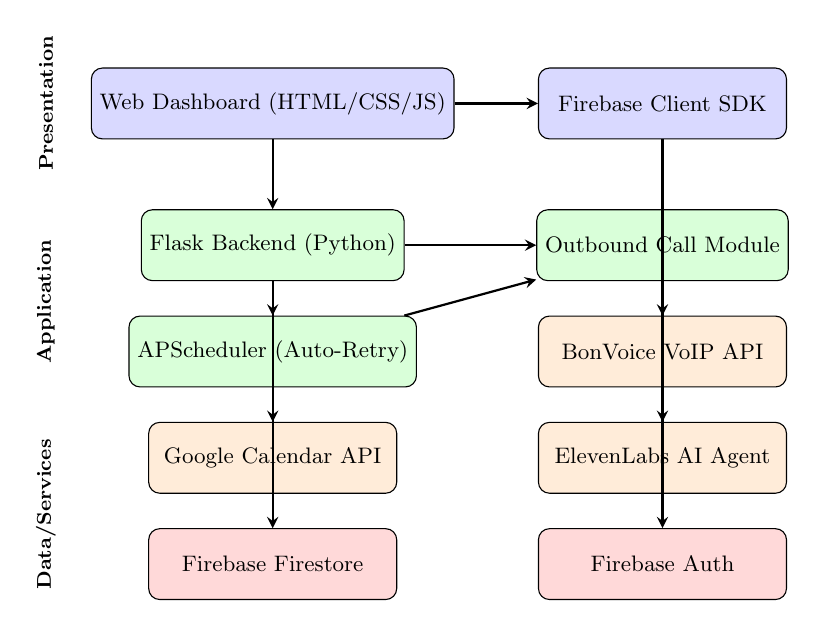
\begin{tikzpicture}[
    box/.style={draw, rounded corners, minimum width=3.5cm, minimum height=1cm, text centered, font=\small},
    arrow/.style={->, thick, >=stealth},
    scale=0.9, transform shape
]

% Presentation Layer
\node[box, fill=blue!15] (ui) at (0,6) {Web Dashboard (HTML/CSS/JS)};
\node[box, fill=blue!15] (firebase_client) at (5.5,6) {Firebase Client SDK};

% Application Layer
\node[box, fill=green!15] (flask) at (0,4) {Flask Backend (Python)};
\node[box, fill=green!15] (outbound) at (5.5,4) {Outbound Call Module};
\node[box, fill=green!15] (scheduler) at (0,2.5) {APScheduler (Auto-Retry)};

% External Services
\node[box, fill=orange!15] (bonvoice) at (5.5,2.5) {BonVoice VoIP API};
\node[box, fill=orange!15] (elevenlabs) at (5.5,1) {ElevenLabs AI Agent};
\node[box, fill=orange!15] (gcal) at (0,1) {Google Calendar API};

% Data Layer
\node[box, fill=red!15] (firestore) at (0,-0.5) {Firebase Firestore};
\node[box, fill=red!15] (fireauth) at (5.5,-0.5) {Firebase Auth};

% Arrows
\draw[arrow] (ui) -- (flask);
\draw[arrow] (ui) -- (firebase_client);
\draw[arrow] (flask) -- (outbound);
\draw[arrow] (flask) -- (scheduler);
\draw[arrow] (outbound) -- (bonvoice);
\draw[arrow] (bonvoice) -- (elevenlabs);
\draw[arrow] (scheduler) -- (outbound);
\draw[arrow] (flask) -- (firestore);
\draw[arrow] (firebase_client) -- (fireauth);
\draw[arrow] (flask) -- (gcal);

% Layer labels
\node[font=\footnotesize\bfseries, rotate=90] at (-3.2,6) {Presentation};
\node[font=\footnotesize\bfseries, rotate=90] at (-3.2,3.2) {Application};
\node[font=\footnotesize\bfseries, rotate=90] at (-3.2,0.2) {Data/Services};

\end{tikzpicture}
\caption{System Architecture of AutoCall Pro}
\label{fig:architecture}
\end{figure}

\subsection{Presentation Layer}

The frontend is built as a single-page-like application using vanilla HTML5, CSS3, and JavaScript. Key UI components include:

\begin{itemize}
    \item \textbf{Login/Signup Page:} Split-panel design with branding and Firebase-authenticated forms supporting email/password registration and login.
    \item \textbf{Dashboard:} Sidebar navigation with three main sections --- Call, Add Lead, and Logs.
    \item \textbf{Call Page:} Single call input and bulk automation controls with live progress bar and streaming call log.
    \item \textbf{Add Lead Page:} Drag-and-drop file upload with Excel/CSV parsing via SheetJS, contact preview table, and Firestore save functionality.
    \item \textbf{Logs Page:} Filterable call log table with date, status, duration, and recording access.
\end{itemize}

\subsection{Application Layer}

The backend is built on \textbf{Flask} (Python 3.x) with the following key modules:

\begin{table}[H]
\centering
\caption{Backend Module Descriptions}
\label{tab:modules}
\begin{tabularx}{\textwidth}{|l|X|}
\hline
\textbf{Module} & \textbf{Description} \\
\hline
\texttt{main.py} & Core Flask application with route definitions, authentication middleware, and API endpoints \\
\hline
\texttt{outbound.py} & Outbound call module handling single calls, bulk calls, and call status checking via BonVoice API \\
\hline
APScheduler & Background job scheduler for automatic retry of failed/unanswered calls at configurable intervals \\
\hline
\end{tabularx}
\end{table}

\subsection{Data Layer}

\textbf{Firebase Firestore} serves as the primary database, storing:
\begin{itemize}
    \item User profiles and authentication state (via Firebase Auth)
    \item Contact/lead records with call status, event IDs, and timestamps
    \item Call logs with recording URLs, duration, and outcome
    \item User settings (retry intervals, calling credentials)
\end{itemize}

\subsection{External Service Integrations}

\begin{table}[H]
\centering
\caption{External Service Integrations}
\label{tab:integrations}
\begin{tabularx}{\textwidth}{|l|l|X|}
\hline
\textbf{Service} & \textbf{Purpose} & \textbf{Integration Method} \\
\hline
BonVoice & VoIP telephony & REST API (outbound-call, call-status, webhooks) \\
\hline
Firebase Auth & User authentication & Client SDK + Admin SDK token verification \\
\hline
Firebase Firestore & Database & Client SDK (frontend) + Admin SDK (backend) \\
\hline
ElevenLabs & AI voice agent & Conversational AI API with agent ID (in progress) \\
\hline
Google Calendar & Meeting scheduling & Calendar API v3 with OAuth 2.0 (planned) \\
\hline
\end{tabularx}
\end{table}

\section{Data Flow}

\subsection{Authentication Flow}
\begin{enumerate}
    \item User submits credentials on login page
    \item Firebase Client SDK authenticates and returns an ID token
    \item Frontend sends ID token to \texttt{/api/auth/verify}
    \item Backend verifies token using Firebase Admin SDK
    \item Session cookie is set for subsequent authenticated requests
\end{enumerate}

\subsection{Outbound Call Flow}
The sequential calling process is illustrated in Algorithm~\ref{alg:sequential}.

\begin{algorithm}[H]
\caption{Sequential Automated Calling}
\label{alg:sequential}
\begin{algorithmic}[1]
\Require List of contacts $C = \{c_1, c_2, \ldots, c_n\}$
\For{each contact $c_i \in C$}
    \State Update $c_i.status \gets$ ``calling''
    \State $result \gets$ \Call{MakeOutboundCall}{$c_i.phone$}
    \If{$result.success$}
        \State $event\_id \gets result.data.event\_id$
        \Repeat
            \State \Call{Sleep}{5 seconds}
            \State $status \gets$ \Call{CheckCallStatus}{$event\_id$}
        \Until{$status.finished = $ \textbf{true}}
        \State Save $status$, $recording\_url$, $duration$ to Firestore
    \Else
        \State Update $c_i.status \gets$ ``failed''
    \EndIf
    \State \Call{Sleep}{2 seconds} \Comment{Gap between calls}
\EndFor
\end{algorithmic}
\end{algorithm}

\subsection{Auto-Retry Flow}

The APScheduler background job runs every 5 minutes and:
\begin{enumerate}
    \item Queries Firestore for contacts with status in \{failed, no-answer, busy, not-connected\}
    \item Checks if the last call attempt was longer ago than the user-configured retry interval
    \item Retries eligible contacts sequentially
    \item Updates Firestore with new status and timestamps
\end{enumerate}

\section{Technology Stack}

\begin{table}[H]
\centering
\caption{Technology Stack Summary}
\label{tab:techstack}
\begin{tabularx}{\textwidth}{|l|X|}
\hline
\textbf{Component} & \textbf{Technology} \\
\hline
Backend Framework & Flask 3.1.0 (Python) \\
\hline
Frontend & HTML5, CSS3, Vanilla JavaScript \\
\hline
Authentication & Firebase Authentication (Email/Password) \\
\hline
Database & Firebase Firestore (NoSQL, real-time) \\
\hline
Telephony & BonVoice VoIP API \\
\hline
AI Voice Agent & ElevenLabs Conversational AI (in progress) \\
\hline
Task Scheduling & APScheduler (BackgroundScheduler) \\
\hline
Excel Parsing & SheetJS (xlsx) --- client-side \\
\hline
HTTP Client & Python Requests 2.32.3 \\
\hline
Environment Config & python-dotenv \\
\hline
Calendar Integration & Google Calendar API v3 (planned) \\
\hline
\end{tabularx}
\end{table}


%%%%%%%%%%%%%%%%%%%%%%%%%%%%%%%%%%%%%%%%%%%%%%%%%
% CHAPTER 4: IMPLEMENTATION
%%%%%%%%%%%%%%%%%%%%%%%%%%%%%%%%%%%%%%%%%%%%%%%%%
\chapter{Implementation}

\section{Project Structure}

The project follows a clean, modular structure:

\begin{lstlisting}[language={}, caption={Project Directory Structure}, label={lst:structure}]
AutoCall-Pro/
|-- main.py                 # Flask app, routes, auth, scheduler
|-- outbound.py             # Outbound call module (BonVoice API)
|-- requirements.txt        # Python dependencies
|-- firebase.json           # Firebase service account credentials
|-- firebase_config.json    # Firebase client configuration
|-- .env                    # Environment variables (API keys)
|-- templates/
|   |-- index.html          # Login/Signup page
|   |-- dashboard.html      # Main dashboard
|-- static/
|   |-- css/
|   |   |-- styles.css      # Login page styles
|   |   |-- dashboard.css   # Dashboard styles
|   |-- js/
|       |-- script.js       # Login page logic (Firebase Auth)
|       |-- dashboard.js    # Dashboard logic (calls, leads, logs)
\end{lstlisting}

\section{Authentication Module}

Authentication is implemented using a dual-layer approach:

\begin{enumerate}
    \item \textbf{Client-side:} Firebase Authentication SDK handles user registration and login via email/password. Upon successful authentication, the SDK provides an ID token.
    \item \textbf{Server-side:} The Flask backend verifies the ID token using Firebase Admin SDK. A session cookie is set for stateful request authentication.
\end{enumerate}

A custom \texttt{@login\_required} decorator protects all API routes:

\begin{lstlisting}[language=Python, caption={Authentication Decorator}, label={lst:auth}]
def login_required(f):
    @wraps(f)
    def decorated(*args, **kwargs):
        token = get_token_from_request()
        if not token:
            if request.path.startswith("/api/"):
                return jsonify({"error": "Authentication required"}), 401
            return redirect(url_for("login_page"))
        decoded = verify_token(token)
        if not decoded:
            if request.path.startswith("/api/"):
                return jsonify({"error": "Invalid or expired token"}), 401
            return redirect(url_for("login_page"))
        request.user = decoded
        return f(*args, **kwargs)
    return decorated
\end{lstlisting}

\section{Outbound Call Module}

The \texttt{outbound.py} module provides three core functions:

\subsection{Single Call (\texttt{make\_outbound\_call})}

Makes a single outbound call via the BonVoice API:
\begin{itemize}
    \item Sanitizes the destination phone number (removes spaces, dashes, parentheses)
    \item Sends a POST request to \texttt{/outbound-call} with API key authentication
    \item Returns success status with \texttt{event\_id} for tracking
    \item Handles timeout, connection errors, and API-specific error codes
\end{itemize}

\subsection{Call Status Checking (\texttt{check\_call\_status})}

Polls the BonVoice API for call progress:
\begin{itemize}
    \item Sends GET request to \texttt{/call-status/\{event\_id\}}
    \item Returns normalized status, finish state, recording URL, and duration
    \item Status lifecycle: initiated $\rightarrow$ initialized $\rightarrow$ answered $\rightarrow$ in-progress $\rightarrow$ completed/hangup/ended
\end{itemize}

\begin{table}[H]
\centering
\caption{Call Status Mapping}
\label{tab:statusmap}
\begin{tabular}{|l|l|l|}
\hline
\textbf{BonVoice Status} & \textbf{UI Display} & \textbf{Firestore Status} \\
\hline
initiated / initialized & Ringing & calling \\
answered / in-progress & On call & calling \\
completed / hangup / ended & Success & called \\
no-answer & Failed & no-answer \\
failed & Failed & failed \\
\hline
\end{tabular}
\end{table}

\subsection{Bulk Calling (\texttt{make\_bulk\_calls})}

Iterates through a contact list and calls each sequentially, returning aggregate statistics (total, initiated, failed).

\section{Lead Management Module}

Lead management is handled entirely on the client-side with Firestore persistence:

\begin{enumerate}
    \item \textbf{File Upload:} Supports Excel (.xlsx, .xls) and CSV files via drag-and-drop or file browser.
    \item \textbf{Parsing:} SheetJS library extracts data client-side, identifying \texttt{name} and \texttt{phone} columns.
    \item \textbf{Validation:} Phone numbers are validated for format and length; duplicates are flagged.
    \item \textbf{Preview:} Parsed contacts are displayed in a table with valid/invalid counts.
    \item \textbf{Save:} Valid contacts are batch-written to Firestore under the user's UID.
\end{enumerate}

\section{Auto-Retry Scheduler}

The APScheduler module provides configurable automatic retry:

\begin{lstlisting}[language=Python, caption={Auto-Retry Scheduler Configuration}, label={lst:scheduler}]
scheduler = BackgroundScheduler(timezone='UTC')
scheduler.add_job(
    auto_retry_failed_calls,
    trigger='interval',
    minutes=5,
    id='auto_retry_job',
    replace_existing=True,
)
scheduler.start()
\end{lstlisting}

Key features:
\begin{itemize}
    \item Checks every 5 minutes for contacts with retryable statuses
    \item Respects user-configured retry intervals (30 min to 24 hours)
    \item Updates contact status to ``calling'' before retry attempt
    \item Records retry success/failure with timestamps
\end{itemize}

\section{REST API Design}

\begin{table}[H]
\centering
\caption{REST API Endpoints}
\label{tab:api}
\begin{tabularx}{\textwidth}{|l|l|X|}
\hline
\textbf{Method} & \textbf{Endpoint} & \textbf{Description} \\
\hline
POST & /api/auth/verify & Verify Firebase ID token, set session cookie \\
\hline
POST & /api/auth/logout & Clear session cookie \\
\hline
GET & /api/auth/session & Check authentication status \\
\hline
GET & /api/user/profile & Get authenticated user profile \\
\hline
POST & /api/outbound/call & Make single outbound call \\
\hline
GET & /api/outbound/call-status/:id & Check call status by event ID \\
\hline
POST & /api/outbound/bulk & Make bulk outbound calls \\
\hline
POST & /api/settings/retry-interval & Save retry interval setting \\
\hline
\end{tabularx}
\end{table}


%%%%%%%%%%%%%%%%%%%%%%%%%%%%%%%%%%%%%%%%%%%%%%%%%
% CHAPTER 5: CURRENT RESULTS AND PROGRESS
%%%%%%%%%%%%%%%%%%%%%%%%%%%%%%%%%%%%%%%%%%%%%%%%%
\chapter{Current Results and Progress}

\section{Completed Modules}

As of the current progress report date, the following modules have been fully implemented and tested:

\subsection{User Authentication}

The Firebase-based authentication system is fully functional with:
\begin{itemize}
    \item Email/password registration with form validation
    \item Secure login with Firebase ID token verification
    \item Session management via HTTP-only cookies (1-hour expiry)
    \item Automatic redirect for unauthenticated users
    \item Password strength indicator during signup
\end{itemize}

\subsection{Dashboard Interface}

The responsive web dashboard provides:
\begin{itemize}
    \item Collapsible sidebar with navigation (Call, Add Lead, Logs)
    \item Mobile-responsive design with overlay navigation
    \item User profile display with sign-out functionality
    \item System status indicator
\end{itemize}

\subsection{Single and Bulk Outbound Calling}

The calling module supports:
\begin{itemize}
    \item Single call initiation with phone number input
    \item Sequential bulk calling with live progress bar
    \item Real-time call status polling (5-second intervals)
    \item Live call log with timestamped status updates
    \item Start/Stop/Continue controls for bulk campaigns
    \item Success/failure/pending counters
\end{itemize}

\subsection{Lead Upload and Management}

The lead management system supports:
\begin{itemize}
    \item Drag-and-drop Excel/CSV file upload
    \item Client-side parsing with SheetJS
    \item Contact preview with validation indicators
    \item Batch save to Firestore with user association
    \item Real-time lead list synchronization
    \item Individual and bulk lead deletion
\end{itemize}

\subsection{Auto-Retry Scheduling}

The background scheduler is operational with:
\begin{itemize}
    \item Automatic retry every 5-minute check cycle
    \item Configurable retry interval (30 min to 24 hours)
    \item Per-user retry interval settings stored in Firestore
    \item Status-based filtering (failed, no-answer, busy, not-connected)
    \item Age-based retry eligibility checking
\end{itemize}

\section{In-Progress Modules}

\subsection{ElevenLabs AI Agent Integration}

The ElevenLabs Conversational AI integration is under active development. The planned implementation involves:
\begin{itemize}
    \item User configures their ElevenLabs API key and Agent ID via the dashboard
    \item Each outbound call is connected to the ElevenLabs agent
    \item The agent dynamically uses lead information (company name, contact name, business details) to personalize the conversation
    \item Call recordings and transcriptions are captured and stored
\end{itemize}

\subsection{Google Calendar Integration}

When the AI agent detects meeting interest during a call:
\begin{itemize}
    \item System will use Google Calendar API to create an event
    \item Google Meet link will be automatically generated
    \item Calendar invite will be sent to the prospect
    \item Meeting details will be logged in Firestore
\end{itemize}

\subsection{Transcription and Summary}

Planned features for call intelligence:
\begin{itemize}
    \item Audio recording storage via BonVoice
    \item Automatic transcription using speech-to-text services
    \item AI-generated conversation summaries
    \item Sentiment analysis and lead scoring
\end{itemize}

\section{System Functional Summary}

\begin{table}[H]
\centering
\caption{Module Completion Status}
\label{tab:progress}
\begin{tabular}{|l|c|l|}
\hline
\textbf{Module} & \textbf{Status} & \textbf{Completion} \\
\hline
User Authentication (Firebase) & \checkmark & 100\% \\
Web Dashboard (Login + Dashboard) & \checkmark & 100\% \\
Single Outbound Call & \checkmark & 100\% \\
Bulk Sequential Calling & \checkmark & 100\% \\
Call Status Tracking & \checkmark & 100\% \\
Lead Upload (Excel/CSV) & \checkmark & 100\% \\
Lead Management (Firestore) & \checkmark & 100\% \\
Auto-Retry Scheduler & \checkmark & 100\% \\
Call Logs Page & \checkmark & 90\% \\
ElevenLabs AI Agent & $\circ$ & 30\% \\
Google Calendar + Meet & $\circ$ & 10\% \\
Transcription \& Summarization & $\circ$ & 10\% \\
Analytics Dashboard & $\circ$ & 0\% \\
\hline
\end{tabular}
\end{table}


%%%%%%%%%%%%%%%%%%%%%%%%%%%%%%%%%%%%%%%%%%%%%%%%%
% CHAPTER 6: CONCLUSION AND FUTURE WORK
%%%%%%%%%%%%%%%%%%%%%%%%%%%%%%%%%%%%%%%%%%%%%%%%%
\chapter{Conclusion and Future Work}

\section{Summary of Progress}

This progress report presents the design and partial implementation of \textbf{AutoCall Pro}, a cloud-based automated outbound calling system with AI voice agent capabilities. The core platform infrastructure has been successfully built and tested, including:

\begin{itemize}
    \item A secure, Firebase-authenticated web application with a responsive dashboard
    \item Complete outbound calling infrastructure via BonVoice VoIP API with real-time status tracking
    \item Lead management with Excel/CSV bulk upload and Firestore persistence
    \item Sequential automated calling with live progress monitoring
    \item Intelligent auto-retry scheduling for failed calls
    \item RESTful API architecture connecting all components
\end{itemize}

The system currently functions as a fully operational automated calling platform. The remaining work focuses on integrating the AI conversation layer (ElevenLabs) and CRM automation features (Google Calendar, transcription, analytics).

\section{Future Work}

The following tasks are planned for completion:

\begin{enumerate}
    \item \textbf{ElevenLabs Conversational AI Integration:} Connect the ElevenLabs agent to each outbound call, enabling dynamic, personalized AI-driven conversations. This includes passing lead context (company name, details) to the agent for each call.

    \item \textbf{Google Calendar and Meet Integration:} Implement OAuth 2.0 flow for Google Calendar access. When the AI agent detects meeting interest, automatically create calendar events with Google Meet links.

    \item \textbf{Call Transcription and Summarization:} Implement audio-to-text transcription for call recordings. Use LLM-based summarization to generate concise call summaries with key action items.

    \item \textbf{Analytics and Reporting Dashboard:} Build campaign analytics with metrics including call success rate, average call duration, conversion rate, and time-based trends.

    \item \textbf{Multi-Provider Telephony Support:} Extend the outbound module to support Twilio alongside BonVoice, allowing users to choose their preferred telephony provider.

    \item \textbf{Dynamic Knowledge Base:} Allow users to upload product/service documents that the AI agent can reference during calls for accurate, contextual responses.

    \item \textbf{Testing and Evaluation:} Conduct systematic testing with real calling scenarios, measure call quality, conversion rates, and user satisfaction.
\end{enumerate}

\section{Expected Contributions}

Upon completion, this thesis will contribute:
\begin{itemize}
    \item An integrated, open-architecture platform for AI-powered outbound sales automation
    \item A practical implementation bridging conversational AI, VoIP telephony, and CRM workflows
    \item Insights into the effectiveness of AI voice agents for outbound sales compared to traditional methods
\end{itemize}


%%%%%%%%%%%%%%%%%%%%%%%%%%%%%%%%%%%%%%%%%%%%%%%%%
% BIBLIOGRAPHY
%%%%%%%%%%%%%%%%%%%%%%%%%%%%%%%%%%%%%%%%%%%%%%%%%
\bibliographystyle{plain}
\bibliography{references}

\end{document}
